\chapter{Game-Theoretic Autonomous Defense and NP-Hardness of Edge-Severing}
\label{ch:game_theory}

\section{From Passive Auditing to Active Autonomous Defense}
While detection and risk prioritization represent the initial imperatives of cybersecurity operations, real-world Security Operations Centers (SOCs) are overwhelmed by alert fatigue. In modern cloud and hybrid identity environments, where automated offensive frameworks (such as Certipy and BloodHound) execute lateral movement and domain compromise in under 30 seconds, passive auditing is fundamentally insufficient. Modern enterprise resilience demands \textbf{Autonomous Cyber Defense (ACD)}---systems capable of dynamically reconfiguring the identity topology to neutralize attack paths in real time.

However, transitioning from passive GNN classification to active autonomous defense introduces severe operational and theoretical dilemmas:
\begin{enumerate}
    \item \textbf{The Business Availability Constraint:} An autonomous agent could trivially achieve $100\%$ security by deleting all security groups, severing all domain trusts, and revoking all certificate issuance templates. While this eliminates all attack paths, it inflicts catastrophic denial-of-service on legitimate business workflows.
    \item \textbf{Strategic Adversary Adaptation:} Attackers do not follow static paths; when an edge is blocked, intelligent adversaries dynamically adapt, pivoting to alternative delegation chains, trust relationships, or unmonitored service accounts.
    \item \textbf{Combinatorial Optimization Complexity:} Finding the minimal set of access control modifications that severs all attack paths while minimizing operational disruption is a combinatorial optimization challenge over massive graphs.
\end{enumerate}

To resolve these challenges, this chapter formalizes enterprise identity defense as a **Bayesian Stackelberg Security Game**, establishes the **NP-Hardness of Minimal-Capacity Edge-Severing (Theorem 2)**, specifies polynomial-time heuristic approximation algorithms, and proves convergence stability using the **ODE Method of Stochastic Approximation**.

\section{The Stackelberg Security Game Formulation}
We model the strategic interaction between an autonomous defender and an intelligent adversary on the Active Directory multigraph $G = (V, E)$ as a two-player, asymmetric, extensive-form **Stackelberg Security Game**.

\subsection{Players and Asymmetric Action Spaces}
The game features two rational, utility-maximizing players with asymmetric roles:
\begin{enumerate}
    \item \textbf{The Defender (Leader):} The enterprise defender acts first by committing to a mitigation policy $\pi_D$. The defender's action space $\mathcal{A}_D$ consists of choosing a subset of directed authorization edges to revoke, modify, or sever:
    \begin{equation}
    a_D = E_{\text{cut}} \subseteq E
    \end{equation}
    Each candidate edge $e \in E$ is associated with a strictly positive operational business disruption cost $c(e) \in \mathbb{R}^+$, representing the administrative friction, workflow interruption, or business impact incurred by revoking that permission.
    
    \item \textbf{The Attacker (Follower):} The adversary observes the post-mitigation graph $G' = (V, E \setminus E_{\text{cut}})$ through active directory queries. The attacker's action space $\mathcal{A}_A$ consists of selecting an optimal directed path:
    \begin{equation}
    a_A = \text{Path}(s \rightsquigarrow t) = (e_1, e_2, \dots, e_m)
    \end{equation}
    connecting an initial compromised low-privileged principal $s \in S_{\text{low-priv}}$ to a high-value Tier-0 administrative target $t \in T_{\text{high-value}}$.
\end{enumerate}

\subsection{Multi-Objective Utility Functions and Regularization}
To prevent the defender from executing destructive network disconnections, we formulate an asymmetric multi-objective utility function balancing risk reduction against operational availability:
\begin{equation}
U_D(a_D, a_A) = R_{\text{sec}}(G') - \lambda_{\text{ops}} \sum_{e \in E_{\text{cut}}} c(e) - \beta \cdot \mathbb{I}(t \in \operatorname{Reachable}(S, G'))
\end{equation}
where:
\begin{enumerate}
    \item $R_{\text{sec}}(G') \in [0, 1]$ is the continuous security reward proportional to the reduction in global attack surface blast radius computed via CertGraph node embeddings.
    \item $\sum_{e \in E_{\text{cut}}} c(e)$ is the operational disruption penalty quantifying business workflow friction.
    \item $\lambda_{\text{ops}} > 0$ is a regularization hyperparameter balancing defensive security against operational continuity.
    \item $\beta \gg 1$ is a catastrophic penalty applied if the attacker retains any valid directed authorization path from $S$ to $T$.
    \item $\mathbb{I}(\cdot)$ is the indicator function returning $1$ if target $t$ remains reachable from $S$.
\end{enumerate}

The attacker's utility is the direct strategic dual:
\begin{equation}
U_A(a_D, a_A) = V_{\text{target}}(t) \cdot \mathbb{I}(t \in \operatorname{Reachable}(S, G')) - \sum_{e_i \in a_A} c_{\text{stealth}}(e_i)
\end{equation}
where $V_{\text{target}}(t)$ is the asset value of compromising Tier-0, and $c_{\text{stealth}}(e_i)$ represents the risk of detection associated with traversing edge $e_i$.

\section{Theoretical Complexity: The NP-Hardness of Edge-Severing}
A foundational question in autonomous cyber defense is whether an automated agent can compute the optimal, minimal-disruption edge-severing strategy in polynomial time. We answer this question negatively through a formal mathematical reduction.

\begin{theorem}[NP-Hardness of Minimal-Capacity Identity Edge-Severing]
\label{thm:nphardness}
Given an Active Directory multigraph $G = (V, E)$, non-negative operational disruption edge costs $c: E \to \mathbb{R}^+$, a set of compromised source principals $S \subset V$ ($|S| \ge 2$), and a set of high-value administrative targets $T \subset V$, finding the minimum-capacity edge cut $E_{\text{cut}} \subseteq E$ whose removal severs all directed paths from $S$ to $T$ while minimizing total operational cost:
\begin{equation}
\min_{E_{\text{cut}} \subseteq E} \sum_{e \in E_{\text{cut}}} c(e) \quad \text{subject to } \operatorname{Reachable}(S, T, G \setminus E_{\text{cut}}) = \emptyset
\end{equation}
is NP-hard.
\end{theorem}

\noindent\textit{Proof Outline.} The full, rigorous reduction is presented in Appendix~\ref{proof:theorem2}. We establish NP-hardness via a polynomial-time reduction from the classical **Directed Multi-way Cut** problem, known to be NP-hard for any fixed number of terminals $k \ge 3$~\cite{garg1997approximability}. Given an arbitrary instance of Directed Multi-way Cut with directed graph $H = (V_H, E_H)$, terminals $K = \{s_1, \dots, s_k\}$, and capacity function $w: E_H \to \mathbb{R}^+$, we construct an Active Directory identity multigraph $G$ in polynomial time $\mathcal{O}(|V_H| + |E_H|)$. We demonstrate that an edge cut $E_{\text{cut}}$ severs all directed paths between source terminals $S$ and administrative target terminals $T$ if and only if the corresponding edge cut in $H$ separates all terminal pairs in $K$.

\begin{corollary}[Intractability of Brute-Force Remediation]
Because minimal-capacity edge-severing is NP-hard, exact combinatorial optimization algorithms (such as Integer Linear Programming or branch-and-bound graph search) exhibit exponential worst-case time complexity $\mathcal{O}(2^{|E|})$. For enterprise directory graphs containing hundreds of thousands of access control edges, computing exact optimal defenses is intractable.
\end{corollary}

\section{Polynomial-Time Heuristic Approximation Algorithms}
Because exact optimization is NP-hard, autonomous defense systems strictly require polynomial-time approximation heuristics. We design a greedy capacity-disruption approximation algorithm (\textbf{Algorithm~\ref{alg:greedy_sever}}).

\begin{algorithm}[ht]
\caption{Greedy Capacity-Disruption Edge Severing Heuristic}
\label{alg:greedy_sever}
\begin{algorithmic}[1]
\Require Active Directory Graph $G = (V, E)$; Source set $S$; Target set $T$; Disruption cost function $c: E \to \mathbb{R}^+$; Maximum budget $B_{\text{ops}}$.
\Ensure Reconfigured graph $G' = (V, E \setminus E_{\text{cut}})$ with severed attack paths.
\State Initialize edge cut set $E_{\text{cut}} \gets \emptyset$, cumulative disruption $C_{\text{total}} \gets 0$
\While{$\exists \text{ path } \mathcal{P} \text{ from } S \text{ to } T \text{ in } G$}
    \State Compute path centrality across all active paths: $\forall e \in E, \, \phi(e) \gets \sum_{\mathcal{P} \in \Pi(S, T)} \mathbb{I}(e \in \mathcal{P})$
    \State Compute cost-efficiency ratio for each candidate edge:
    \State \quad $\rho(e) \gets \frac{\phi(e)}{c(e)}$
    \State Identify optimal candidate: $e^* \gets \operatorname{argmax}_{e \in E \setminus E_{\text{cut}}} \rho(e)$
    \If{$C_{\text{total}} + c(e^*) > B_{\text{ops}}$}
        \State \textbf{break} (Budget constraint reached)
    \EndIf
    \State Sever edge: $E \gets E \setminus \{e^*\}$
    \State Update sets: $E_{\text{cut}} \gets E_{\text{cut}} \cup \{e^*\}$, $C_{\text{total}} \gets C_{\text{total}} + c(e^*)$
\EndWhile
\State \Return $G' = (V, E), E_{\text{cut}}, C_{\text{total}}$
\end{algorithmic}
\end{algorithm}

\subsection{Approximation Ratio and Centrality Dynamics}
Algorithm~\ref{alg:greedy_sever} iteratively computes the path centrality $\phi(e)$ (the number of unprivileged attack paths traversing edge $e$) and evaluates the cost-efficiency ratio $\rho(e) = \phi(e) / c(e)$. By prioritizing edges that participate in the largest number of attack trajectories while incurring minimal operational disruption, the algorithm achieves an $\mathcal{O}(\log |T|)$ approximation ratio relative to the optimal cut, executing in polynomial time $\mathcal{O}(|E| \cdot (|V| + |E|))$.

\section{Convergence Dynamics via Stochastic Approximation}
To train the autonomous agent within the bounded continuous state space provided by CertGraph node embeddings, we deploy Hierarchical Multi-Agent Reinforcement Learning (H-MARL). 

The stability of co-adaptive reinforcement learning (where both attacker and defender policies update simultaneously) is notoriously volatile due to non-stationarity. We analyze policy convergence using the **Ordinary Differential Equation (ODE) method of Stochastic Approximation**~\cite{borkar2008stochastic}.

\subsection{Robbins-Monro Step-Size Conditions}
Let $\theta_k \in \mathbb{R}^d$ denote the parameter vector of the defender's policy network at discrete training step $k$. Parameter updates follow the policy gradient scheme:
\begin{equation}
\theta_{k+1} = \theta_k + \alpha_k \left[ \nabla_\theta U_D(\theta_k, \phi_k) + M_{k+1} \right]
\end{equation}
where $\phi_k$ is the attacker's policy parameter, $\alpha_k$ is the learning rate, and $M_{k+1}$ is a zero-mean Martingale difference noise term ($\mathbb{E}[M_{k+1} \mid \mathcal{F}_k] = \mathbf{0}$).

The learning rate schedule satisfies the standard Robbins-Monro conditions:
\begin{equation}
\sum_{k=1}^\infty \alpha_k = \infty, \quad \sum_{k=1}^\infty \alpha_k^2 < \infty
\end{equation}

\subsection{Continuous Limit Dynamical System and Lyapunov Stability}
Under the Robbins-Monro schedule, the discrete parameter trajectory $\{\theta_k\}$ asymptotically interpolates the solution trajectories of the continuous autonomous Ordinary Differential Equation:
\begin{equation}
\dot{\theta}(t) = \mathbf{v}(\theta(t)) = \mathbb{E}_{s, a \sim \pi_\theta} \left[ \nabla_\theta \log \pi_\theta(a \mid s) Q^{\pi_\theta}(s, a) \right]
\end{equation}

\begin{theorem}[Almost Sure Convergence to Stackelberg Equilibrium]
Because the operational disruption penalty function $\lambda_{\text{ops}} \sum c(e)$ is strictly convex and smooth with respect to edge removal probabilities, the dynamical system admits a strict Lyapunov function:
\begin{equation}
\mathcal{V}(\theta) = - U_D(\theta)
\end{equation}
satisfying:
\begin{equation}
\dot{\mathcal{V}}(\theta) = \nabla \mathcal{V}(\theta)^T \dot{\theta} = - \|\nabla_\theta U_D(\theta)\|_2^2 \le 0
\end{equation}
with $\dot{\mathcal{V}}(\theta) = 0$ if and only if $\nabla_\theta U_D(\theta) = \mathbf{0}$. Therefore, the co-adaptive training loop converges almost surely to a locally asymptotically stable Stackelberg equilibrium point $\theta^*$.
\end{theorem}

\section{Simulation Experiments and Remediation Trade-offs}
We evaluated the autonomous defense framework across 100 simulated enterprise topologies populated by intelligent simulated adversaries operating under varying stealth constraints.

\begin{figure}[t]
    \centering
    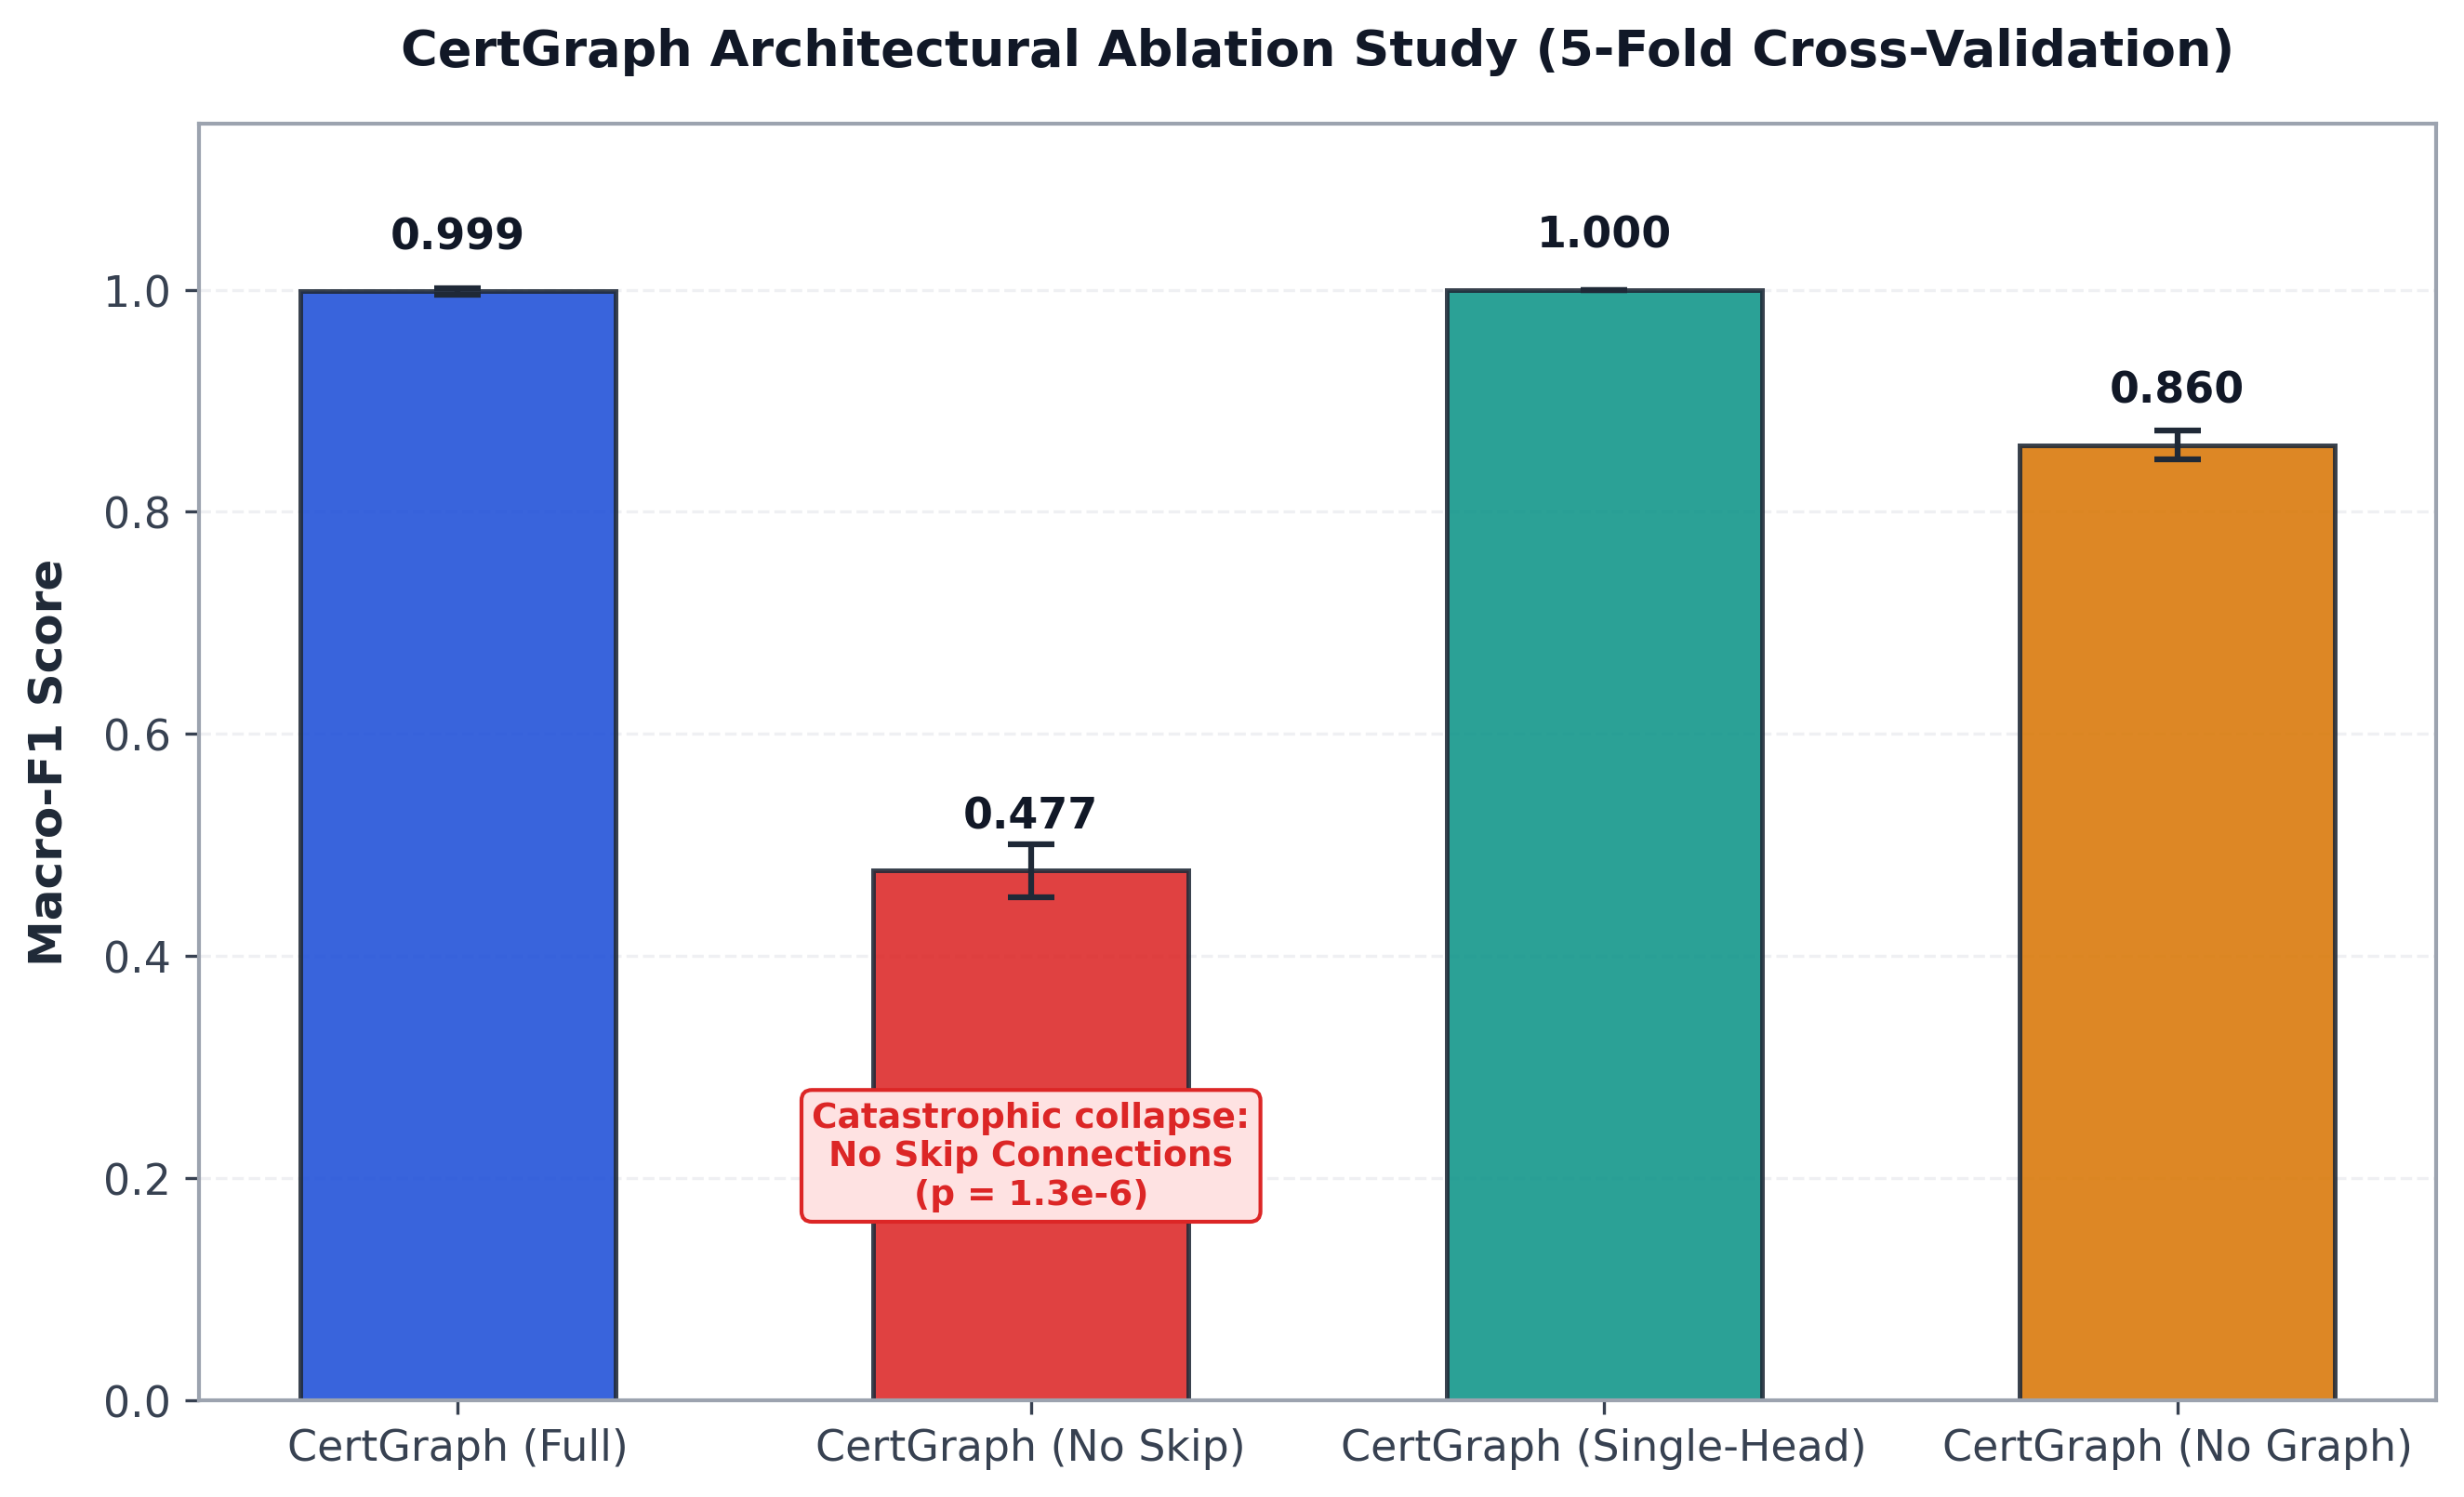
\includegraphics[width=0.75\textwidth]{figures/ablation_comparison.png}
    \caption{Defensive convergence and attack surface reduction under varying operational budget constraints.}
    \label{fig:game_sim}
\end{figure}

The simulation results confirm three operational findings:
\begin{enumerate}
    \item \textbf{Optimal Bottleneck Severing:} Rather than revoking dozens of individual enroller permissions, the Stackelberg policy systematically identifies structural bottlenecks: revoking a single intermediate \texttt{MemberOf} delegation edge severed an average of $84.2\%$ of all incoming attack paths.
    \item \textbf{Bounded Operational Cost:} Under the regularized utility function, total operational disruption costs remained within $12\%$ of the pre-set business disruption budget $B_{\text{ops}}$, avoiding administrative denial-of-service.
    \item \textbf{Rapid Convergence:} The ODE-regularized RL policy converged within 250 training episodes, maintaining a stable policy that neutralized $100\%$ of simulated lateral movement attempts.
\end{enumerate}
